% !TEX root = ../main.tex

\chapter{Results Evaluation}

This chapter discusses results provided by the developed system and how they answer the questions posed at the beginning of this project.

\section{Examined Entity}

The entity that will examined is a company called Gamestop. Gamestop is an American video game, consumer electronics, and gaming merchandise retailer. It is the largest video game retailer worldwide.

\begin{figure}[h!]
    \centering
    
\includegraphics[width=15cm,height=4cm,keepaspectratio]{resultsEvaluation/gamestop.png}
    \caption{Gamestop Logo}
    \label{fig:gamestop}
\end{figure}

The main reason for choosing this company is due to the fact that it has historically been a relatively stable company. However, an interesting sentiment fueled phenomenon happened recently. In January of 2021, the company stock prices increased by 1,500\% over the course of two weeks due to a short squeeze mainly attributed to the members of a subreddit, r/wallstreetbets. Reddit is a social news aggregation, web content rating, and discussion website, and a subreddit is a channel within this website which specialises in a given topic. In this case a subreddit dedicated to stocks with high market risk. This seems to indicate that the stock prices of Gamestop were heavily driven by sentiment. Making this an exceptional case-study for this project.

\section{Descriptive Statistics}

The first step towards understanding the dataset is to understand each of the columns by themselves. This first step that may be used is to create an outline of the dataset using descriptive statistics, alongside a graph. This lays out the data in such a way were time is not an element and simply the general trends of the data can be understood. A part of this analysis is to attempt to understand whether these general trends have remained consistent. Therefore, various time spans are examined alongside the dataset as a whole. The timespans examined here are the entire dataset and the past year worth of data. The full set of data looked at is stored in the appendix \ref{appendix:descriptiveStatistics}.

\subsection{Price Columns}

The cloumns which give the most amount of information are:
\begin{itemize}
    \item Closing Prices
    \item 1 Day Returns
\end{itemize}

\begin{figure}[h!]
    \centering
    \subfigure[]{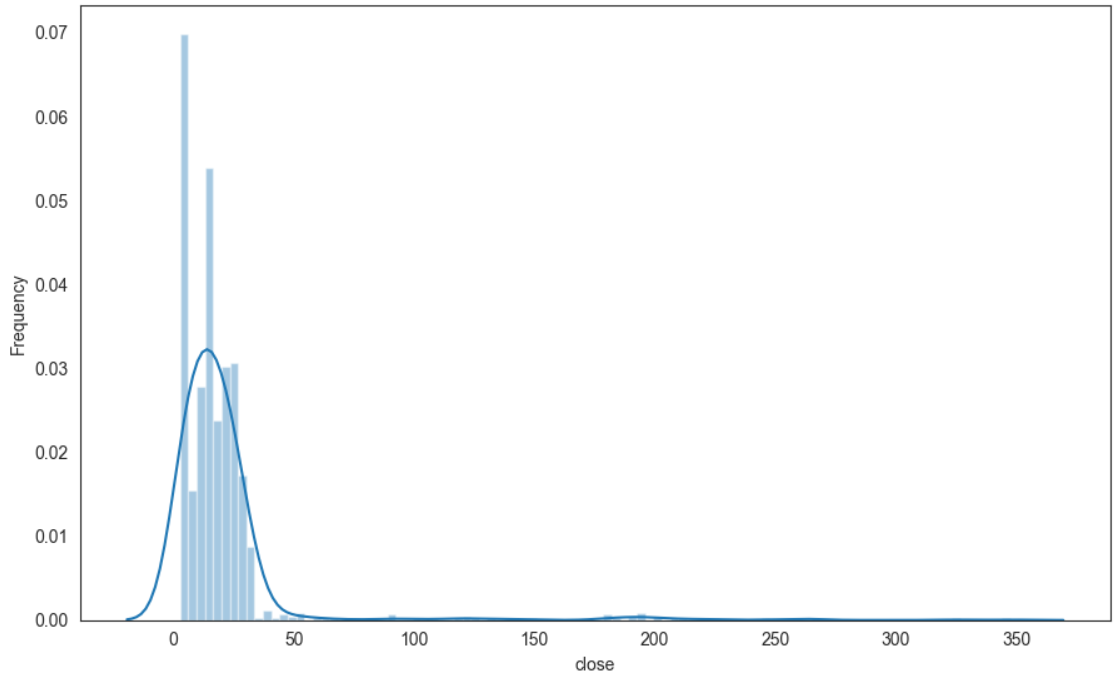
\includegraphics[width=0.49\textwidth,height=4cm]{resultsEvaluation/closeDescMax.png}}
    \subfigure[]{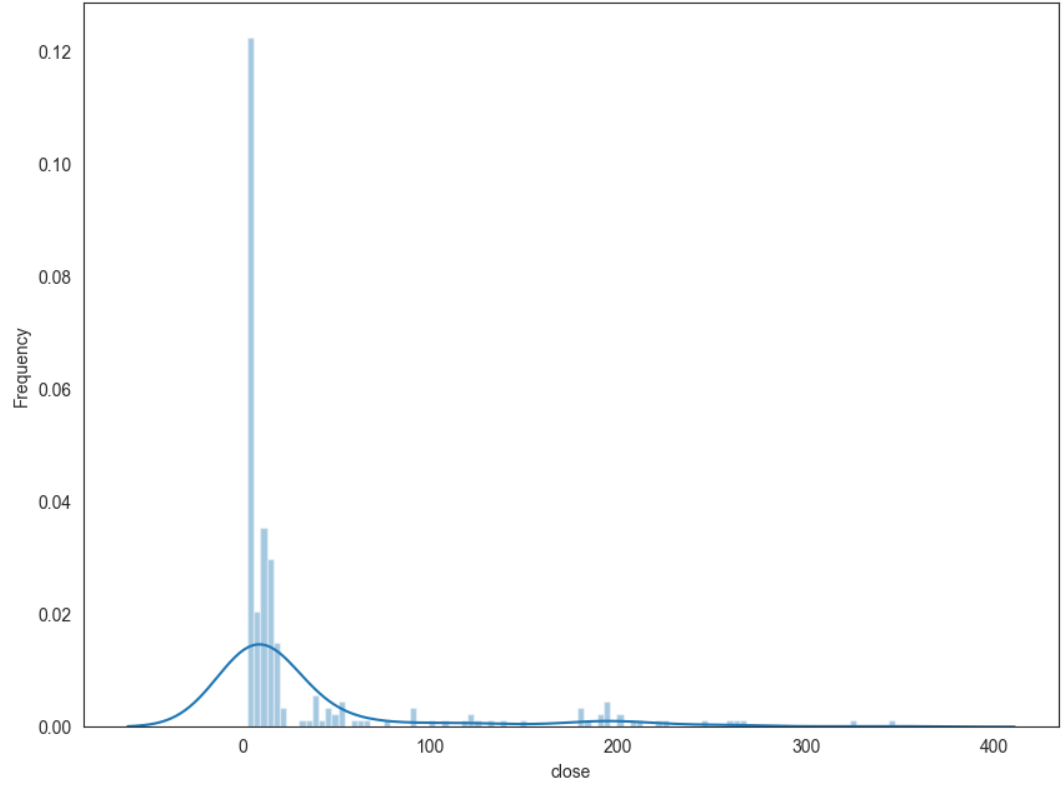
\includegraphics[width=0.49\textwidth,height=4cm]{resultsEvaluation/closeDesc1.png}}
    \caption{Closing Prices (a) entire dataset (b) last year of data}
    \label{fig:closeDesc}
\end{figure}

The first column examined is the closing price column. The initial observations from the overall dataset are:
\begin{itemize}
    \item There is a heavy left skew, confirmed with a skewness value of 6.0809, evidenced with a mean of 20.2554 when the standard deviation is 30.5661 and the minimum value is 2.8 while the maximum value is 347.51
    \item There are long tails, confirmed with a kurtosis value of 43.0012 and a range of 344.71 when the standard deviation is 30.5661
    \item There is a large concentration of points in the one area, making it unimodal, evidenced by a standard error of 0.8618
\end{itemize}
The dataset which includes only the last year of datapoints compares in the following ways. The overall value of the closing prices has increased to having a mean of 35.3204 from 20.2554. However the most common values do lie in the same are as the mode went from 4.14 to 4.44, indicating tht in general the price stayed the same. The median went from 15.22 to 10.22, actually decreasing a little bit, indicating that the much higher highs were balanced by much lower lows. The heavy left skew is maintained, it is however diminished with a new skewness value of 2.5837. This can partially be explained by the maximum and minimum values being the same, and the large amount of curve flattening seen by the standard error increasing to 4.0341 from 0.8618, the standard variance increasing to 4117.2946 from 935.0304. Similarly, the tails are still long given the kurtosis value of 6.1112, and the maintenance of the same range. However, the tails have more values within. All of this combined indicates that in the last year the stock's closing price has been far more volatile that usual, with the highest highs and lowest lows in the range examined. It seem that it has generally incread in value given the new mean. However, it is still hovering around the same price given the mode and median.

\begin{figure}[h!]
    \centering
    \subfigure[]{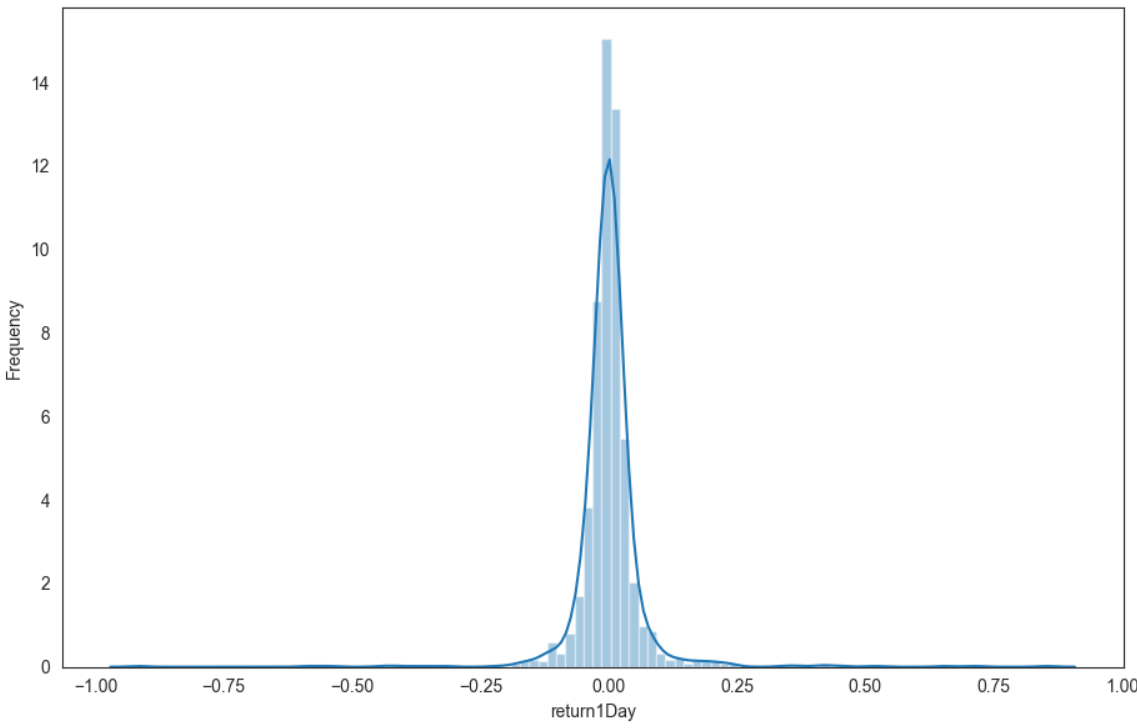
\includegraphics[width=0.49\textwidth,height=4cm]{resultsEvaluation/1returnDescMax.png}}
    \subfigure[]{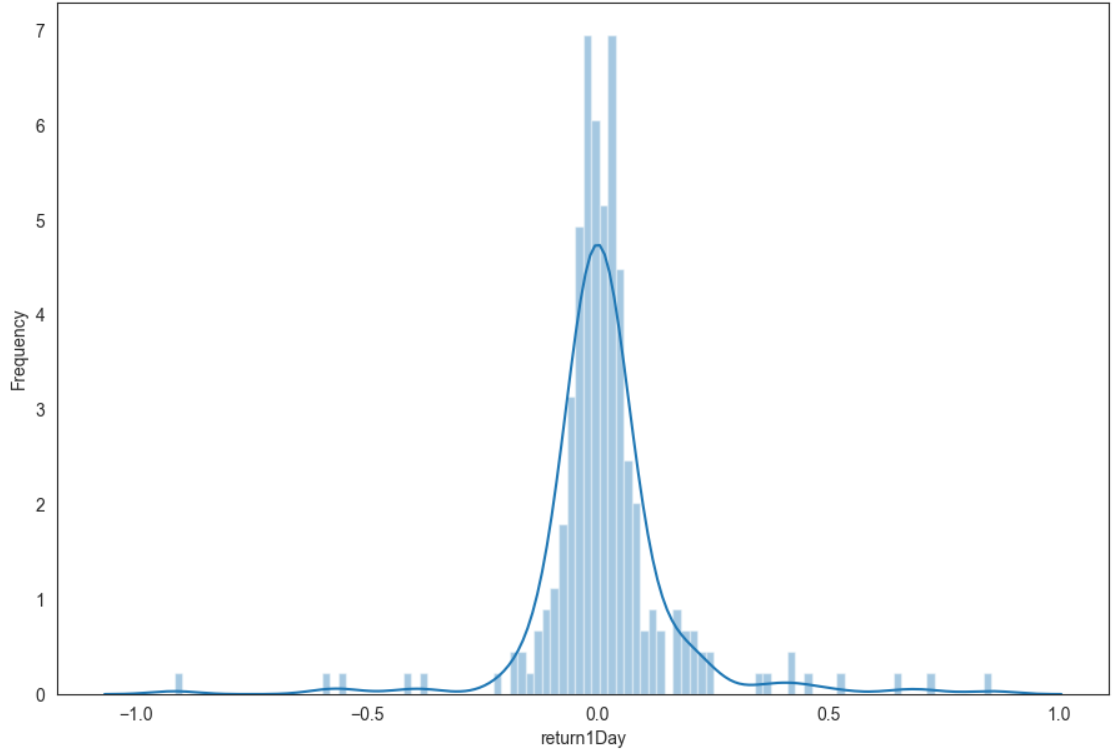
\includegraphics[width=0.49\textwidth,height=4cm]{resultsEvaluation/1returnDesc1.png}}
    \caption{1 Day Returns (a) entire dataset (b) last year of data}
    \label{fig:1returnDesc}
\end{figure}

The 1 day returns column is also examined. The initial observations are:
\begin{itemize}
    \item There is little to no skew, confirmed with a skewness value of 0.7638
    \item There are long tails, given the kurtosis value of 51.5650 and evidenced with the range of 1.7700 with a standard deviation of 0.0755
    \item There is a large concentration of points in the one area, making it unimodal, and evidenced with a standard error of 0.0021
\end{itemize}
The examination of the full dataset confirms the points made for closing prices. The mean, mode and median are all increased to 0.0162, 0.0053 and 0.0223 from 0.0014, 0.0 and 0.0. Indicating higher returns than over the entire dataset, however, this is marginal. Similarly as with closing proces the skewness remains quite similar, to 0.7638 from 0.3239, where the decrease may be attributd to the increased flatness of the curve, seen by the standard error increase to 0.0096 from 0.0021. As well as this the tails are kept long, seen in the kurtosis value of 12.8680, and the same range being maintained. This information confirms the points laid out for closing prices.

\subsection{Sentiment Columns}

\begin{figure}[h!]
    \centering
    \subfigure[]{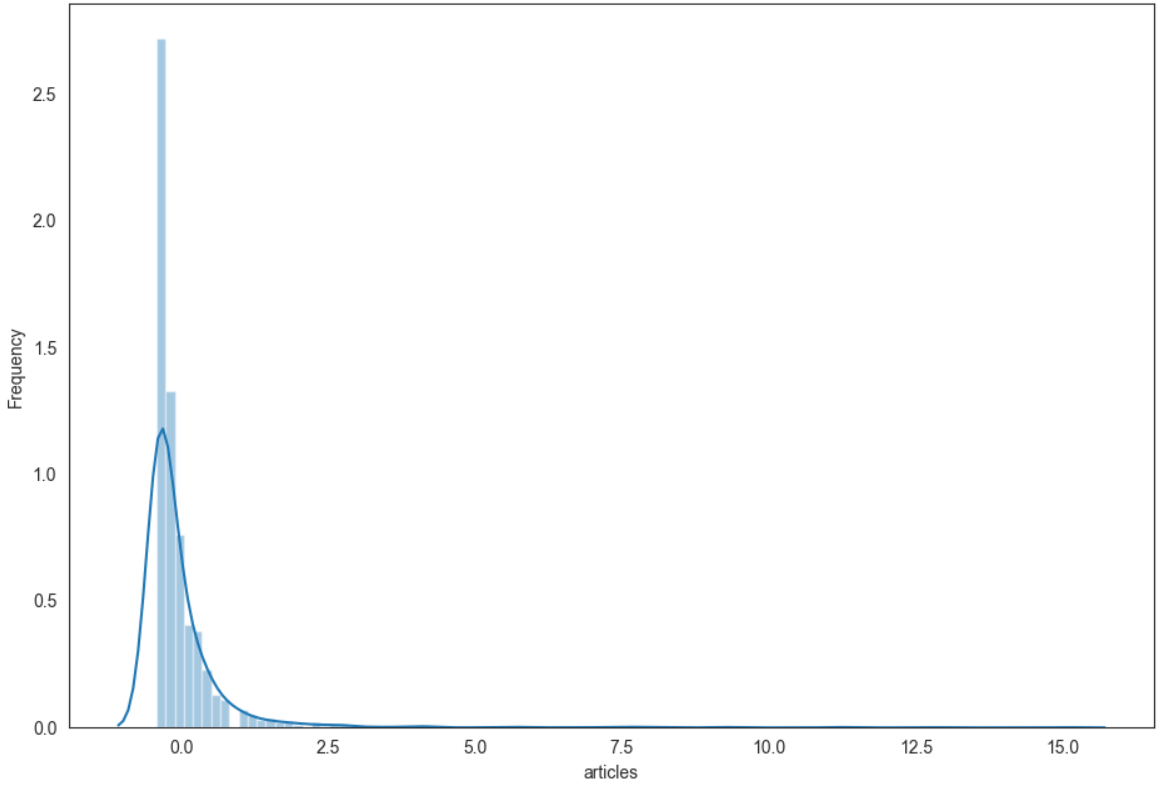
\includegraphics[width=0.49\textwidth,height=4cm]{resultsEvaluation/articleDescMax.png}}
    \subfigure[]{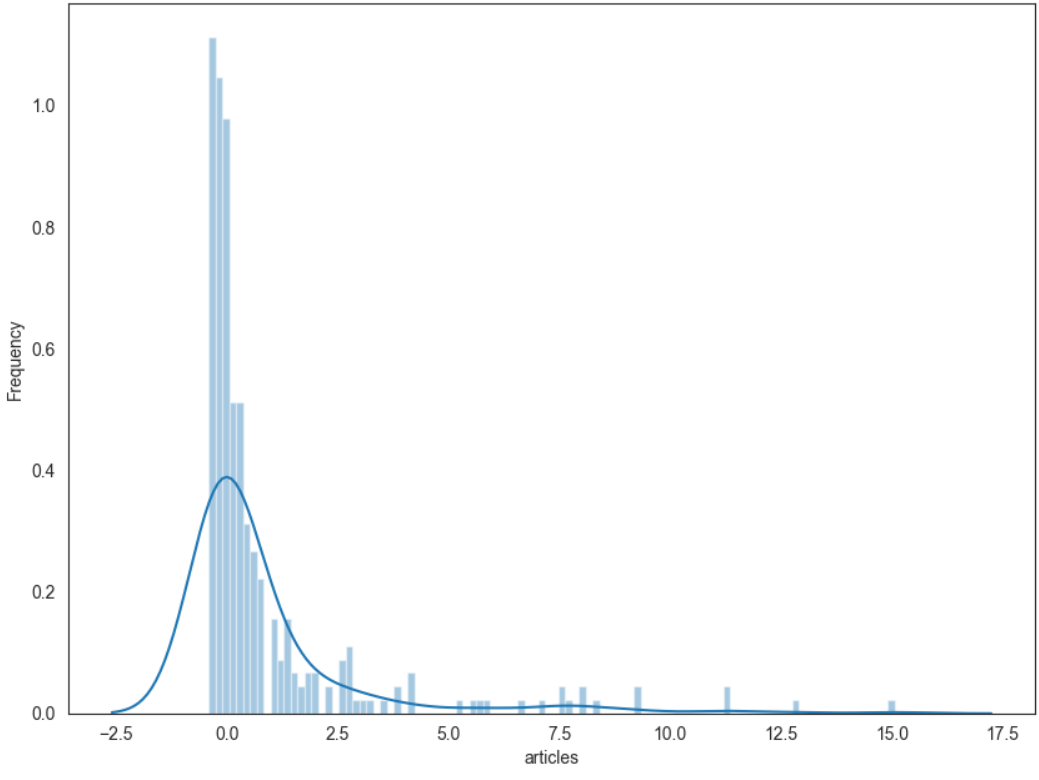
\includegraphics[width=0.49\textwidth,height=4cm]{resultsEvaluation/articleDesc1.png}}
    \caption{Article Volume (a) entire dataset (b) last year of data}
    \label{fig:articleDesc}
\end{figure}

The first column examined from the sentiment columns is the article volume column. The initial observations from the full dataset are:
\begin{itemize}
    \item There is a heavy left skew, confirmed by the skewness value of 7.3609
    \item There are long tails, given by the kurtosis value of 73.7692 and the range of 15.4788 and standard deviation of 1.0
    \item There is a large concentration of points in one area, making it unimodal, and evidenced with a standard error of 0.0220
\end{itemize}
The dataset which only takes into account one year is then considered. The mean and median are raised to 0.8623 and 0.1096 from 0.0 and -0.2422, meanwhile the mode is maintaned constant at -0.4181. This indicates that there are more higher values, however, most of them are still concentrated in the same area. The other difference to point out is that flattening of the curve, indicated in the change of standard error to 0.1325 from 0.0220. The tailness maintained but slightly decreased due to the flattening of the curve, seen in the change of kurtosis to 12.2162 from 73.7692. The changes indicate that in the last year there was was more variation in the number of article towards the high-end, however, the majority of points remain the same. This aligns with what is seen in the prices and returns, which indicates some correlation between the two aspects.

\begin{figure}[h!]
    \centering
    \subfigure[]{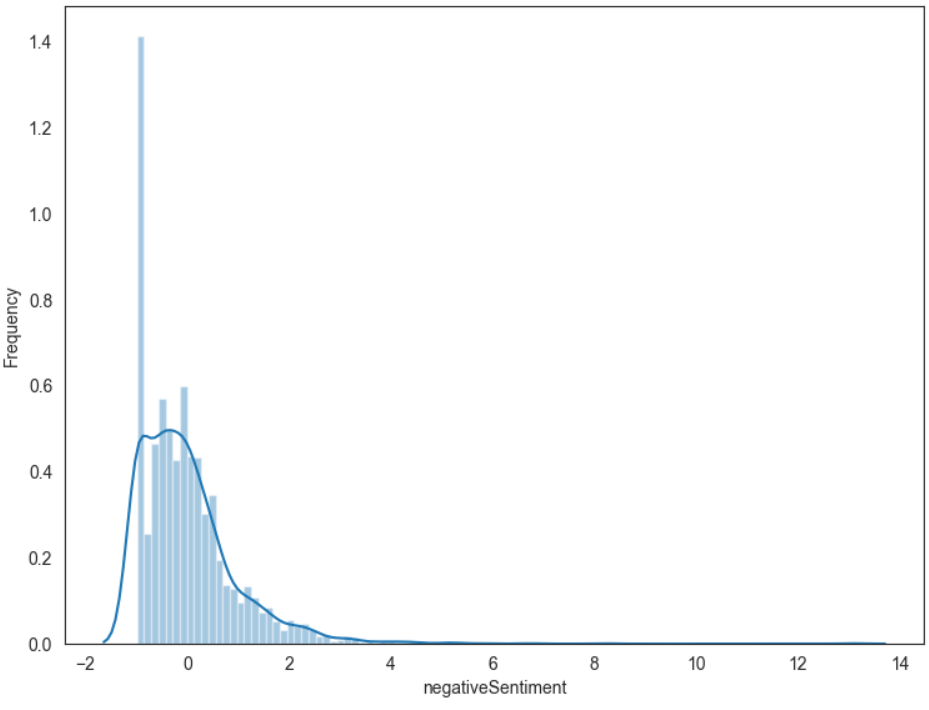
\includegraphics[width=0.49\textwidth,height=4cm]{resultsEvaluation/negativeDescMax.png}}
    \subfigure[]{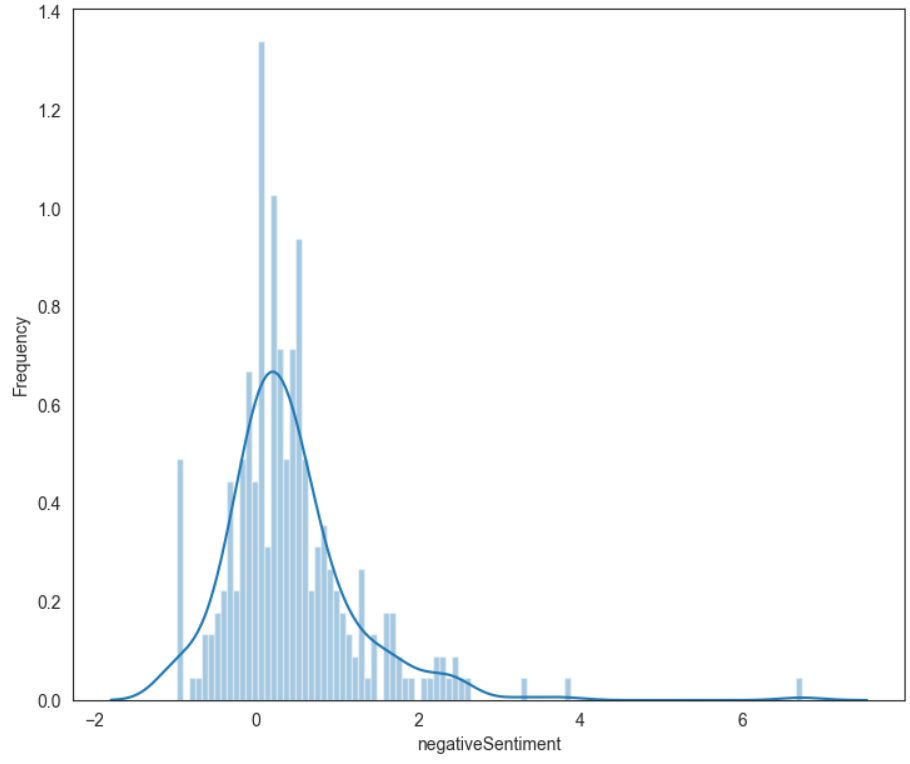
\includegraphics[width=0.49\textwidth,height=4cm]{resultsEvaluation/negativeDesc1.png}}
    \caption{Negative Sentiment (a) entire dataset (b) last year of data}
    \label{fig:negativeDesc}
\end{figure}

The next column examined is the negative sentiment column. The positive and negative sentiment column behave very similarly. So only one of these is examined. The initial observations are:
\begin{itemize}
    \item There is a left skew, confirmed by the skewness value of 2.7791
    \item There are long tails, given by the kurtosis value of 19.5138 and the range of 14.05 and standard deviation of 0.9998
    \item The data is concentrated around one area, making it unimodal, and evidenced with a standard error of 0.0220
\end{itemize}
The 1 year dataset compare in the following ways. The mean, median and mode all increase to 0.4129, 0.27 and 0.08 from 0.0001, -0.17 and -0.99. This indicates a general increase in negative sentiment in the last year. The curve flattened a small amount in the year given the change of standard error to 0.0489 from 0.0220. Unlike the rest of the examined columns however, the range of data is significantly decreased to 7.72 from 14.05, where the minimum remained the same at -0.99, and the maximum decreased from 13.06 to 6.73. These items seem to indicate that the general sentiment was more negative more regularly, however, it never reached the extremes that it previously had. It is interesting to note that a similar pattern occur when positive sentiment is examined. This seems to indicate that when there is more volatility in the market, and a larger amount of articles, the sentiment is generally higher, negative and positive.

It is important to note that preceding information indicates that the examination is conditional on the timespan examined for this dataset. This is due to the fact that the descriptive statistics change significantly depending on the timespan chosen.

\section{Auto Correlation}

This step in understanding the dataset continues the understanding of columns by themselves. However, it examines the relationship of the cloumns with themselves. It does this by finding the correlation of a column entry with a previous entry given a lag time. For example if the lag is 5, it will find the correlation with 5 entries prior, i.e. 5 days before. This is important to understand whether previous days have any correlation, and potentially an effect on the current day.

TODO
\begin{center}
\begin{tabular}{ c c }
\hline
\multicolumn{2}{|c|}{Closing Price AutoCorrelation with entire dataset} \\
\hline
1 day lag & 0.9411935591590456 \\
2 day lag & 0.9109376954243168 \\
3 day lag & 0.8588675104961536 \\
4 day lag & 0.7892956691827954 \\
5 day lag & 0.7580804740115362
\end{tabular}
\end{center}

- Not over 90\% correlation
- Does not -> volatile stock

\begin{center}
\begin{tabular}{ c c }
\hline
\multicolumn{2}{|c|}{1 Day Return AutoCorrelation with entire dataset} \\
\hline
1 day lag & 0.010044065231783677 \\
2 day lag & 0.13420635746867923 \\
3 day lag & 0.17706335839486953 \\
4 day lag & -0.23281554097728582 \\
5 day lag & 0.0305722042951903
\end{tabular}
\end{center}

- Mean Reversal
    - Increase then negative
- Add up to > 0, long term growth
    - Seen in inconsistency with prices autocorrelation

\begin{center}
\begin{tabular}{ c c }
\hline
\multicolumn{2}{|c|}{Article Volume AutoCorrelation with entire dataset} \\
\hline
1 day lag & 0.7086866740522393 \\
2 day lag & 0.5051901969956358 \\
3 day lag & 0.3913458079243162 \\
4 day lag & 0.35884587791576666 \\
5 day lag & 0.4345743036499016
\end{tabular}
\end{center}

\begin{center}
\begin{tabular}{ c c }
\hline
\multicolumn{2}{|c|}{Positive Sentiment AutoCorrelation with entire dataset} \\
\hline
1 day lag & 0.2189007770374344 \\
2 day lag & 0.16697193082109396 \\
3 day lag & 0.13939070288175473 \\
4 day lag & 0.1571263190342898 \\
5 day lag & 0.12675439356211746
\end{tabular}
\end{center}

\begin{center}
\begin{tabular}{ c c }
\hline
\multicolumn{2}{|c|}{Negative Sentiment AutoCorrelation with entire dataset} \\
\hline
1 day lag & 0.1936071341220439 \\
2 day lag & 0.14727144175440102 \\
3 day lag & 0.13880100344429427 \\
4 day lag & 0.10022996242458204 \\
5 day lag & 0.19026511070278398
\end{tabular}
\end{center}

\section{Return to Sentiment Correlation}

TODO graphs

\begin{center}
\begin{tabular}{ c c }
\hline
\multicolumn{2}{|c|}{1 Day Return to Negative Sentiment Correlation with entire dataset} \\
\hline
0 day lag & -0.005749086829293921 \\
1 day lag & 0.04767256694150456 \\
2 day lag & 0.031817132474997706 \\
3 day lag & 0.04737555379831079 \\
4 day lag & -0.007019212993683423 \\
5 day lag & 0.043130405239089696
\end{tabular}
\end{center}

\begin{center}
\begin{tabular}{ c c }
\hline
\multicolumn{2}{|c|}{Negative Sentiment to 1 Day Return Correlation with entire dataset} \\
\hline
0 day lag & -0.005749086829293921 \\
1 day lag & -0.01986514709858617 \\
2 day lag & -0.01863445341486425 \\
3 day lag & -0.031901855696982465 \\
4 day lag & -0.04423692450337006 \\
5 day lag & -0.04438304347685678
\end{tabular}
\end{center}

- Return -> Negative Sentiment
    - Mean Reversal?
- Negative Sentiment -> Negative Return

\section{Vector Autoregression}

\section{}
autoregression vs ml

\section{Results Evaluation Summary}

This chapter uses the results provided by the system to explore the questions posed for this project.